% O modelo inteiro em figuras (06/11/2026, pedido do autor). NÃO é parte do TG:
% o autor analisa antes de decidir se e onde entra. Figuras TikZ desta pasta
% (fig-panorama, fig-fluxo), compiladas pelo Makefile. Dados e conferência:
% dados/resultados/modelo_completo_2026-11-06/LEIAME.md.
\documentclass[11pt,a4paper]{article}
\usepackage[T1]{fontenc}
\usepackage[brazilian]{babel}
\usepackage{mathptmx}
\usepackage[a4paper,margin=2.2cm]{geometry}
\usepackage{graphicx}
\usepackage[font=small,labelfont=bf]{caption}
\usepackage[most]{tcolorbox}
\usepackage[hidelinks]{hyperref}
\setlength{\parskip}{0.45em}
\setlength{\parindent}{0pt}

\definecolor{cesc}{RGB}{220,50,32}
\definecolor{cmod}{RGB}{0,90,181}
\newtcolorbox{ideia}[1][]{colback=cmod!5, colframe=cmod!70, fonttitle=\bfseries, title={#1}, arc=2pt, boxrule=0.6pt}
\newtcolorbox{cuidado}[1][]{colback=cesc!4, colframe=cesc!70, fonttitle=\bfseries, title={#1}, arc=2pt, boxrule=0.6pt}
\newcommand{\arqm}[1]{../../../dados/resultados/modelo_completo_2026-11-06/#1}
\newcommand{\arqr}[1]{../../../dados/resultados/robo_em_acao_2026-10-30/#1}
\input{\arqm{valores.tex}}
\input{\arqr{valores.tex}}

\title{O modelo inteiro em figuras\\[2pt]\large um pregão do começo ao fim e o caminho de dois anos de pregões}
\author{Material de análise, fora do TG}
\date{6 de novembro de 2026}

\begin{document}
\maketitle

Este relatório reúne duas figuras que mostram o robô ARIMA-GARCH inteiro de uma vez. A primeira acompanha um único
pregão, dos fechamentos até a ordem, com as séries e os números que o robô de fato usou. A segunda mostra o que o
modelo fez com todos os pregões de dois anos: quantos o ARIMA mandou para cada lado, quantos o GARCH vetou e onde o robô
terminou. Nada aqui foi colocado no \texttt{tg/}.

As figuras que já existem tratam do modelo por partes. As do TG (Figuras 2, 5 e 6) são fluxogramas genéricos, sem dado.
As da apresentação mostram um método por figura, e a 08 já percorre um pregão em caixas de texto. O que estas
acrescentam é ver as peças juntas, com o desenho de cada série no lugar do número solto.

\section{Um pregão do começo ao fim}

\begin{figure}[p]
\centering
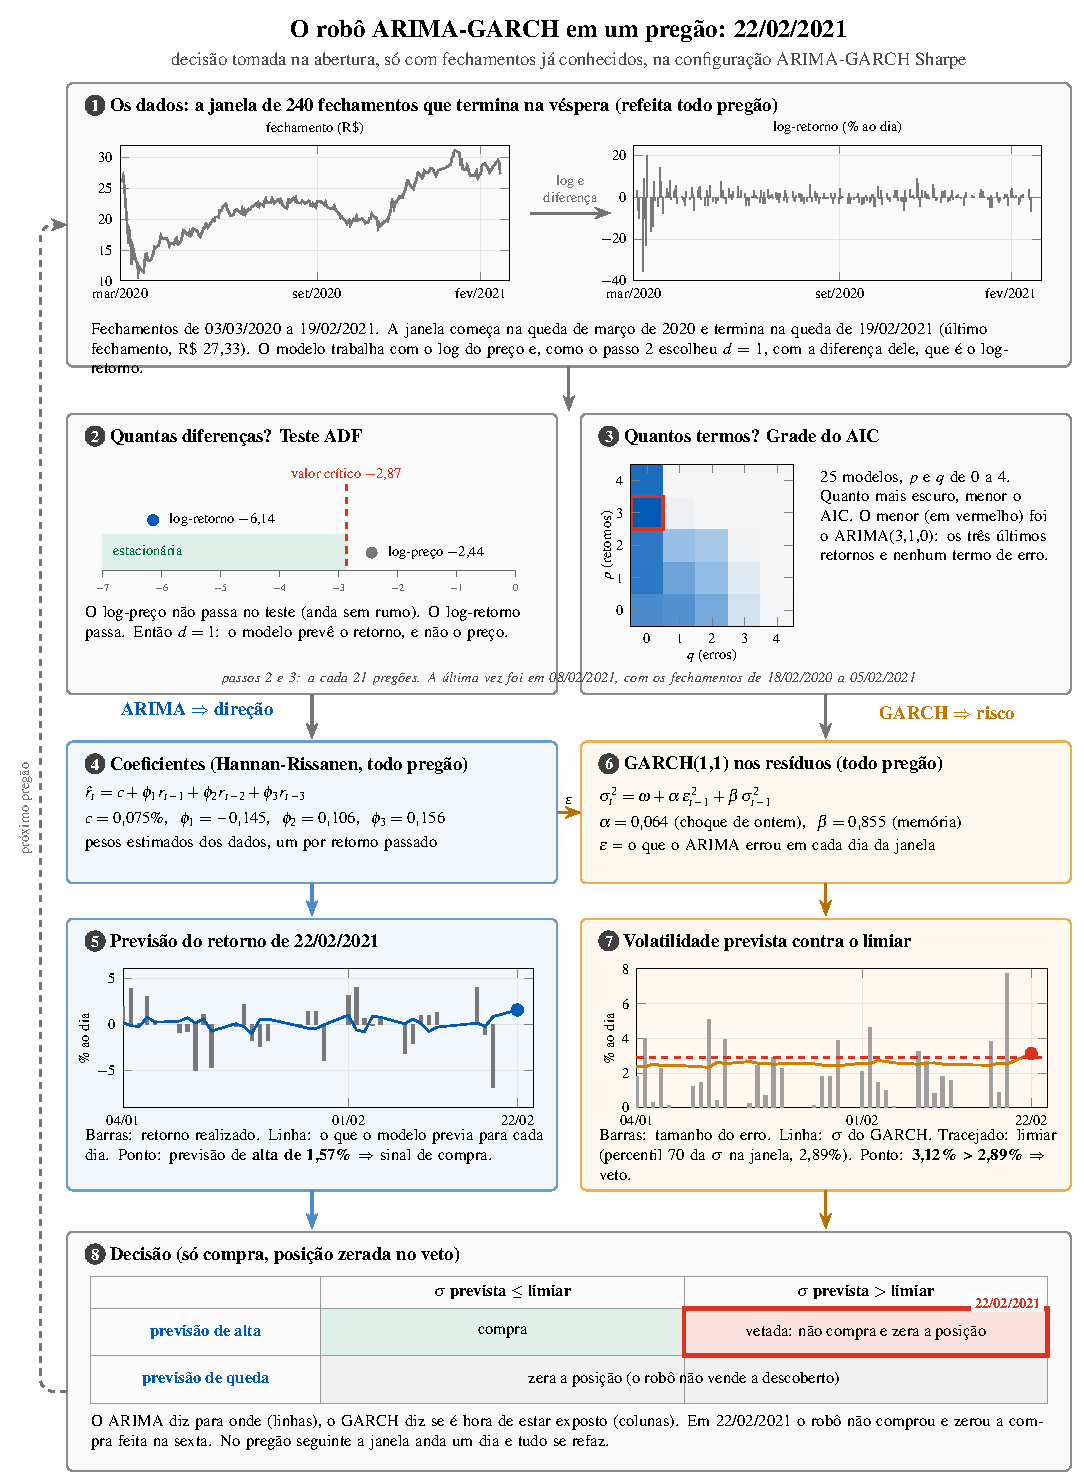
\includegraphics[width=\textwidth]{fig-panorama.pdf}
\caption{O robô ARIMA-GARCH em um pregão (\vSegDia)}
\label{fig:panorama}
\end{figure}

A Figura~\ref{fig:panorama} usa o pregão de \vSegDia, o mesmo da figura 08 da apresentação, em que o ARIMA previu alta e
o GARCH vetou. O exemplo foi escolhido porque mostra as duas partes do modelo discordando. A configuração é a
ARIMA-GARCH Sharpe escolhida na calibração de 2014 a 2016, com janela de 240 pregões, constante, nova escolha de ordens a
cada 21 pregões, GARCH como filtro no percentil~70, só compra e posição zerada no veto.

\begin{ideia}[Como ler, de cima para baixo]
O passo 1 é a matéria-prima: os 240 fechamentos até a véspera e o log-retorno que sai deles. Os passos 2 e 3 escolhem o
formato do modelo e só rodam a cada 21 pregões. O ADF decide quantas diferenças tirar ($d$) e a grade do AIC decide
quantos retornos passados ($p$) e quantos erros passados ($q$) entram. Daí em diante o desenho se divide em duas pistas.
À esquerda, o ARIMA estima os pesos (passo 4) e prevê o retorno do dia (passo 5): é a direção. À direita, o GARCH
recebe os erros do ARIMA, estima como a agitação se propaga (passo 6) e prevê a volatilidade do dia (passo 7): é o
risco. O passo 8 junta as duas respostas numa tabela de quatro casas, e só uma delas é compra. A seta tracejada à
esquerda lembra que tudo se refaz no pregão seguinte.
\end{ideia}

Os números da figura saem de um script novo, \texttt{ferramentas/ModeloCompleto.mq5}, que chama as funções do próprio
robô sobre a mesma janela. Ele refaz a escolha das ordens no pregão da última reseleção (\vSegSel), o ajuste do ARIMA e
do GARCH, a previsão, o limiar e a decisão. Tudo coincide com o que o robô gravou no traço da refação de 05/10/2026:
ordens, coeficientes, $\alpha$, $\beta$, previsão de \vSegPrev\%, volatilidade de \vSegVol\% e limiar de \vSegLim\%
(\texttt{conferencia.txt} na pasta dos dados).

\begin{cuidado}[O que a figura não diz]
É um exemplo escolhido para mostrar o mecanismo, não um resultado médio. O GARCH não previu a queda de 22/02: ele reagiu
ao erro de \vSegUltRes\% da sexta, que o robô perdeu do mesmo jeito, porque estava comprado. Os números do ADF e da grade
do AIC (passos 2 e 3) são da janela da última reseleção, que termina em \vSegSelFim, e não da janela do dia, que é a dos
gráficos do passo 1. A legenda do passo 2 diz isso. Por fim, a janela do dia começa em plena queda de março de 2020, o
que pesa no GARCH desse pregão (ver o relatório \texttt{garch-funcionando}).
\end{cuidado}

\section{O caminho de dois anos de pregões}

\begin{figure}[h]
\centering
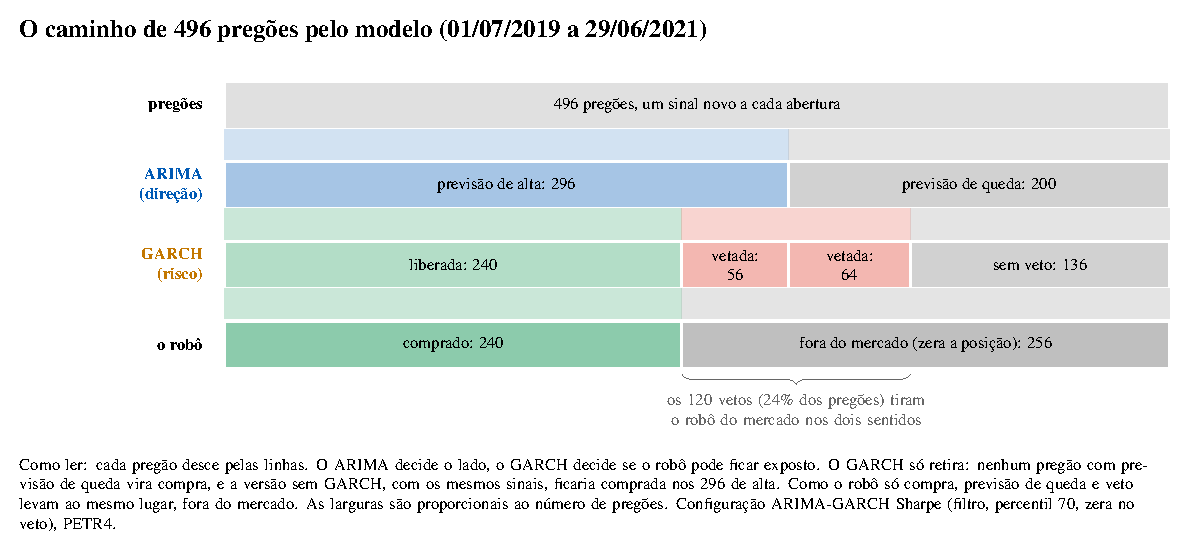
\includegraphics[width=\textwidth]{fig-fluxo.pdf}
\caption{Os \pRN{} pregões de \vRInicio{} a \vRFim{} passando pelo modelo}
\label{fig:fluxo}
\end{figure}

A Figura~\ref{fig:fluxo} conta os pregões do mesmo traço (\vRInicio{} a \vRFim, calmaria, crise da COVID e recuperação)
e mostra por onde cada um passou. As larguras são proporcionais. Em \pRComprasA{} pregões o ARIMA previu alta e em
\pRVendasA, queda. O GARCH vetou \pRVetos{} (\vRVetosPct\%), \pRVetoCompra{} com previsão de alta e \pRVetoVenda{} com
previsão de queda. O robô ficou comprado em \pRCompras{} pregões.

\begin{ideia}[O que a figura deixa claro]
A divisão de papéis aparece sozinha. O ARIMA reparte os pregões entre os dois lados e o GARCH só retira, nunca acrescenta.
E como o robô só compra, a previsão de queda e o veto levam ao mesmo lugar, fora do mercado. Por isso, dos \pRVetos{}
vetos, só os \pRVetoCompra{} com previsão de alta mudaram o que o robô fez. Os outros \pRVetoVenda{} caíram em dias em
que ele já ficaria fora. A versão sem GARCH, com os mesmos sinais, ficou comprada nos \pRComprasA{} pregões de alta.
\end{ideia}

\begin{cuidado}[Contagem não é resultado]
A figura conta pregões, não mede lucro nem queda. Pregões vetados podem ter sido de alta ou de baixa. A figura 13 da
apresentação já mostra que, na queda de março de 2020, as duas versões estavam fora porque o próprio ARIMA deu sinal de
venda, e não por causa do GARCH. As contagens vêm de \texttt{dados/resultados/robo\_em\_acao\_2026-10-30/valores.tex}
e foram recontadas a partir do \texttt{dia\_a\_dia.csv} ao montar a figura (240, 56, 64 e 136, somando 496).
\end{cuidado}

\section{Se for para o TG}

A decisão é do autor. Uma possibilidade é a Figura~\ref{fig:panorama} entrar no Capítulo~II, em ``Implementação dos
modelos'', como a visão de conjunto antes dos detalhes, ou nos slides como a figura de abertura do método. A
Figura~\ref{fig:fluxo} cabe melhor na apresentação, ou no Capítulo~III junto da discussão do veto. Em qualquer dos
casos, o negrito e o tamanho da fonte dentro das figuras teriam de ser revistos pelas normas da FATEC, e o pregão do
exemplo precisaria ser citado no texto.

Para refazer: \texttt{bash ferramentas/scripts/modelo\_completo.sh} (roda o MetaTrader e confere contra o traço) e
\texttt{make} nesta pasta.

\end{document}
